%!TEX TS-program = pdflatex
\documentclass[11pt,ngerman]{beamer}
 
 \usepackage[T1]{fontenc}
 \usepackage{booktabs}
 \usepackage{babel}
 \usepackage{graphicx}
 \usepackage{csquotes}
 \usepackage{xcolor}
 \usepackage{tikz}

\author{Uwe Ziegenhagen}
\title{Synthesizer}
 
 \begin{document}
 
 \begin{frame}

\maketitle
 
 \end{frame}
 
 
\begin{frame}
\frametitle{Inhalt}

\tableofcontents

\end{frame}
 
 \begin{frame}
 \frametitle{Über mich und diese Präsentation}
 
\begin{itemize}
 \item Dr. Uwe Ziegenhagen, IT-Spezialist für Treasury Systeme \item lebe und arbeite in Köln, spiele kein Instrument
 \item Interesse an der Entstehung von elektronischer Musik im Synthesizer
 \item Diese Präsentation: wie funktioniert ein Synthesizer 
 \item Zahlreiche unterschiedliche Quellen, Wikipedia, etc.
\end{itemize}
 \end{frame}
 
\section{Theoretische Grundlagen}

%\subsection{Ton und Klang}

\begin{frame}
\frametitle{Ton}

\begin{itemize}
	\item gleichmäßig und einheitliche Schwingung der Luft, die vom (menschlichen) Gehör wahrgenommen werden kann
	\item anders als ein Impuls (Hammerschlag, Knall)
	\item anders als ein Geräusch (ungleichmäßige Schwingungen und Frequenzen)
\end{itemize}\vspace*{1em}

Einzelne Töne werden charakterisiert nach \vspace*{0.5em}

\begin{itemize}
	\item Tonhöhe (Frequenz, Schwingungen pro Sekunde, Note)
	\item Tondauer (Sekunden oder Notenwert)
	\item Laut-/Tonstärke als Höhe der Amplitude, per Schalldruck in dB oder Lautstärkeangabe
\end{itemize}

\end{frame}


\begin{frame}
\frametitle{Klang}

\begin{itemize}
\item in der physikalischen Akustik: Klang = Ton
\item in der Musiktheorie: das simultane Auftreten mehrerer Töne
\item Gemisch aus:

\begin{itemize}
	\item Grundton (1. Partialton)
	\item Obertönen
	\item Rauschanteilen
	\end{itemize}

\item Grundton bestimmt die wahrgenommene Tonhöhe
\item Obertöne bestimmen die Klangfarbe
\item Obertöne sind üblicherweise die ganzzahligen Vielfache des Grundtons (Kammerton\footnote{Stimmton/Normalton} a\textsuperscript{1} = 440 Hz, a\textsuperscript{2} = 880 Hz, \newline a\textsuperscript{3} = 1320 Hz))
\end{itemize}
\end{frame}

%\subsection{Synthese}

\begin{frame}
\frametitle{Hüllkurven}

\begin{itemize}
\item dienen zur Modellierung des Signalverlaufs
\item meist vier Stufen: A, D, S und R
\end{itemize}
 {\scriptsize
\begin{description}
\item[A] Attack (Anstieg) Durch das Drücken der Taste erhält der Hüllkurvengenerator einen Impuls, die Attack-Phase beginnt. Die Attack-Zeit gibt die Zeit an, in der die Spannung von Null bis auf ihr vorgegebenes Maximum ansteigt. 

\item[D] Decay (Abfall)  Unmittelbar nachdem das Maximum erreicht wurde, beginnt die Decay-Phase. Der Decay-Parameter (Dauer oder Steilheit) legt die Zeit fest, in der die Spannung vom Maximum auf den Sustain-Pegel absinkt.

\item[S] Sustain (Halten)  Der Sustain-Pegel gibt an, wie hoch die Spannung ist (in Prozent des Maximums), während die Taste gehalten wird. 

\item[R] Release (Freigeben) Sobald die Taste losgelassen wird, beginnt die Release-Phase. In der Release-Phase sinkt die Spannung vom gegenwärtigen Pegel auf Null ab. Der Release-Parameter (Dauer oder Steilheit) legt fest, wie lange dieser Vorgang dauert. 

\end{description}
}

\end{frame}

\begin{frame}
\frametitle{ADSR-Hüllkurve (Wikipedia)}

\begin{center}
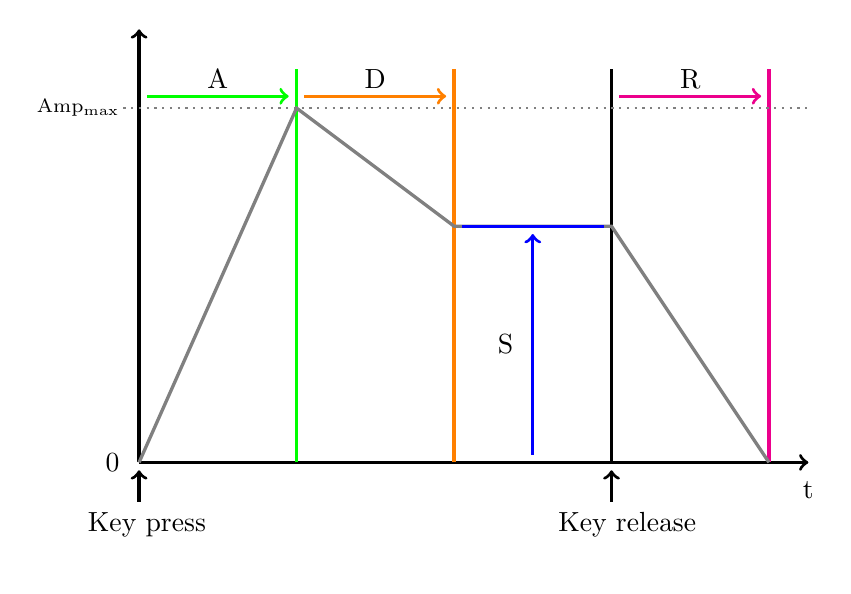
\begin{tikzpicture}
%\draw[step=0.5cm,lightgray,thin] (0,0) grid (10,7);
\draw[very thick, black,->](1,1) -- (9.5,1);
\draw[very thick, black,->](1,1) -- (1,6.5);
\draw[very thick, green,](3,1) -- (3,6);
\draw[very thick, orange,](5,1) -- (5,6);
\draw[very thick, black](7,1) -- (7,6);
\draw[very thick, magenta](9,1) -- (9,6);

\draw[very thick, gray,](1,1) -- (3,5.5) -- (5,4) -- (7,4)--(9,1);
% max amp line
\draw[thick, gray,dotted](0.8,5.5) -- (9.5,5.5);

\draw[very thick, blue,->](6,1.1) -- (6,3.9);

\draw[very thick, green,->](1.1,5.65) -- (2.9,5.65);
\draw[very thick, orange,->](3.1,5.65) -- (4.9,5.65);

\draw[very thick, blue](5.1,4) -- (6.9,4);

\draw[very thick, magenta,->](7.1,5.65) -- (8.9,5.65);

\node[label=left:0] (A) at (1,1) {};
\node[label=below:t] (B) at (9.5,1) {};
\node[label=left:{{\scriptsize Amp\textsubscript{max}}}] (C) at (1,5.5) {};

\node[label=above:A] (D) at (2,5.5) {};
\node[label=above:D] (E) at (4,5.5) {};
\node[label=left:S] (F) at (6,2.5) {};
\node[label=above:R] (G) at (8,5.5) {};

\draw[very thick, black,->](1,0.5) -- (1,0.9);
\draw[very thick, black,->](7,0.5) -- (7,0.9);

\node[label=above:{Key press}] (D) at (1.1,-0.2) {};
\node[label=above:{Key release}] (D) at (7.2,-0.2) {};

\end{tikzpicture}
\end{center}

\end{frame}
 
\section{Synthesizer - Geschichtliches}

\begin{frame}
\frametitle{Geschichtliches I}


\begin{itemize}
\item 1957: RCA Mark II Synthesizer, erster programmierbarer elektronischer Synthesizer, Steuerung über Lochkarten 
\item 1964: erster Moog Synthesizer von Robert Moog, erste VCOs, Envelopes, Noise Generators
\item 1970: Minimoog
\item 1978: Prophet-5 von Sequential Circuits (Dave Smith), erste Verwendung von Mikroprozessoren
\item 1982: MIDI Protokoll
\item 1983: Yamaha DX7, erste Verwendung der FM Synthese, mehr als 100\,000 verkaufte Exemplare
\item 1995: Eurorack Format von Doepfer Musikelektronik
\item 1997: Propellerhead ReBirth und Seer Systems Reality, erste Software Synthesizer
\end{itemize}
\end{frame} 
 
\begin{frame}
\frametitle{Geschichtliches II}


\begin{itemize}
\item 
\item 
\item 
\item 
\item 
\item 
\end{itemize}
\end{frame}
 
 
\section{Arten von Synthesizern}
 
\begin{frame}
\frametitle{Kompakt, Modular, Semi-Modular}

\begin{description}
\item [Kompakt] alles in einem Gerät vorkonfiguriert, keine Möglichkeit, \textit{extern} zu patchen
\item [Semi-Modular] vorkonfiguriert, aber mit Patch-Punkten, um das Gerät zu \enquote{verlassen}
\item [Modular] komplette Kontrolle, wie der Signal-Fluss aussehen soll, aber teuerste Option
\end{description}
\end{frame}




%\section{Kompakte Synthesizer}
 
\begin{frame}
\frametitle{Kompakte Synthesizer}

\begin{itemize}
\item beliebte Geräte: Korg Microkorg, Arturia Microfreak
\end{itemize}
\end{frame}
 
 
 \begin{frame}
 \frametitle{Semi-Modulare Synthesizer}
  
 \begin{itemize}
 \item Beispiele: Roland System-1m, Moog Mother-32, Arturia Microbrute
 \item eigenständige Synthesizer, aber patchbar 
 \item 
 \item 
 \item 
 \item 
 \end{itemize}
 \end{frame}
 
 
 
%\section{Modulare Synthesizer} 
 
\begin{frame}
\frametitle{Voll-Modulare Synthesizer}

\begin{itemize}
\item Synthesizer aus unterschiedlichen Modulen zusammenstellen
\item Im Wesentlichen drei Standards:

\begin{itemize}
	\item Eurorack, mit 3 HE (Höheneinheiten)
	\item Buchla Modular (4 HE)
	\item Moog (5 HE)
\end{itemize}
\item Eurorack hat die größte Verbreitung, veröffentlicht 1996 von Doepfer
\item ModularGrid listet knapp 15\,000 unterschiedliche Eurorack-Module
\item Verbreitung von Buchla und Moog eher gering, Preise \textit{echt} hoch $\Rightarrow$ Fokus daher auf Eurorack
\item Preislich schmerzhaft, unter 1\,000 Euro Gesamtpreis wenig sinnvoll
\end{itemize}
\end{frame} 

\begin{frame}
\frametitle{Eurorack Gehäuse}

\begin{itemize}
\item Gehäuse, das die einzelnen Module aufnimmt
\item Größenangabe in \textit{U} und \textit{HP}
\item 3U = eine Modulreihe, 6U = zwei Modulreihen
\item HP = Horizontal Pitch = 0.2 Zoll bzw. 5.08 mm
\item Leergehäuse 1 U, 84 HP bei ca. 150 Euro
\item dazu noch ca. 100 EUR für Netzteil und Busschiene (Stromversorgung der einzelnen Module)
\item fertige Gehäuse ab 250 Euro
\end{itemize}
\end{frame}

\begin{frame}
\frametitle{Module}

\begin{itemize}
\item In das Eurorack werden dann die einzelnen Module eingesetzt
\item Wichtig: Breite und Einbautiefe, nicht jedes Gehäuse kann jedes Modul aufnehmen
\item Welche Module? 
\begin{itemize}
	\item Ton muss rein: Sequencer/CV \& Midi Interface
	\item Ton muss raus:
	\item Dazwischen: Qual der Wahl! VCOs, Mixer, Effekte
\end{itemize}
\end{itemize}
\end{frame}

 
\section{Links} 
 
\begin{frame}[allowframebreaks]
\frametitle{Linksammlung}


\begin{itemize}
\item \url{de.wikipedia.org/wiki/Subtraktive_Synthese}
\item \url{de.wikipedia.org/wiki/Additive_Synthese}
\item \url{www.amazona.de/was-genau-ist-ein-synthesizer-synthesen-im-ueberblick/}
\item \url{www.bhphotovideo.com/explora/pro-audio/tips-and-solutions/a-guide-to-analog-subtractive-synthesis-with-the-moog-phatty-keyboard}
\item \url{https://www.thomann.de/de/onlineexpert_topic_synthesizer.html}
\item 
\item 
\end{itemize}
\end{frame} 
 
 
 \end{document}